\section{Route planning}
In order to be able to suggest routes to motorists, the system must find the best route available at a given time and day of the week. One could define several quality measures of a good route, but in this case we consider the best route in terms of time, that is, the shortest travel time. The process is known as finding shortest paths in a directed weighted graph, and existing algorithms solve this problem well. In this section we discuss the methods used for finding such shortest paths.

\subsection{A* Heuristic Search}\label{sec:pathfinding}
We use the heuristic search algorithm A* since it is a widely used approach for finding shortest path routes in graphs and can be improved by further preprocessing of the graph as discussed in \chapref{ch:future-work}.

We design the heuristic as an underestimate of the real travel time from a given node to the target node, by letting the heuristic be the travel time of traveling the Euclidean distance at 120 km/h (i.e. the highest speed limit in Beijing) from a given node to the target node.

Let $h(v)$ be the heuristic function:
\begin{align*}
h(v) = &\frac{dist(u,v)}{120 km/h} \qquad u,v \in V
\end{align*}
that computes an underestimate of the travel time from $u$ to $v$ to ensure the graph search proceeds in the correct direction in the graph.

At every expansion of a node, each of the weights of the neighbouring nodes are computed using the weight of the segment that leads from the node being expanded to the neighbour at a particular time of a given day. Each time a node is explored the weight of the current node added to the start time will be used as the time when calculating the weight of each of the neighbouring nodes. The idea is illustrated in \figref{fig:timed-graph}.

\begin{figure}[h]
\centering
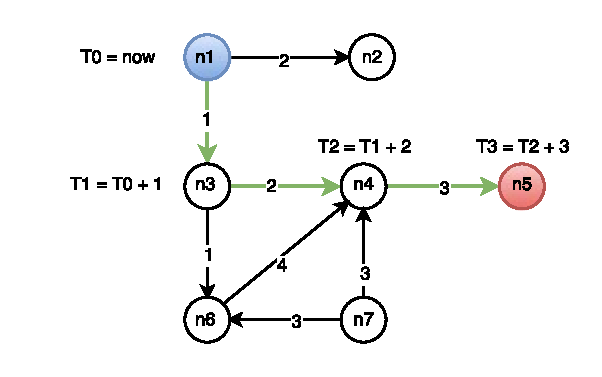
\includegraphics[width=\linewidth]{figures/timed-graph}
\caption{Relative times in path-finding - Numbers on edges are weights in time. Relative time is indicated next to nodes. The green arrows indicate the shortest path found. The weight of each segment is calculated based on the time of the origin node.}
\label{fig:timed-graph}
\end{figure}

%An A* is used to finding a path through the graph. There are other versions of a A* search that are faster then a normal A*, but these do not work with the weight function that are being used. The time complexity of this search is $O(b^n)$ where $b$ is the branching factor and $n$ is the number of nodes in the graph.

%The function is given a start and a goal node, the A* utilise the physical destined between these point as a heuristic to make sure the path it takes goes in the right direction. Then it finds the time and ask the database for the cost of the segments it can travel from the node it's at.

%The reason for using this algorithm over other graph search is that the the time for finding a path is $O(b^{(n/2)})$ where a normal Dijkstra’s takes $O(b^{n})$, where $b$ is the branching factor and $n$ is the number of nodes in the direct graph. Bi-directional also have the benefit of working well when running in paralleled.


% How do we use it?
%By using bi-directional search there is one problem that needs to be address, this is will the search meet op before the whole graph is search. There are more then one way of solving this problem, in this project A* have been chosen for solving this problem. The A* makes sure that the search from the start node wakes a path towards the end node and the other way around for the search that starts from end node.

%By implementing the bi-directional search this way, the worst case running time becomes $O(b^{n})$. The reason for this is that each search is going towards the other search's start node and not it's frontier. The search will stop if one of the two searches hits a node that the other search have visited.

\subsection{Weight function}\label{sec:weight-function}
The weight of road segments is the travel time required to travel along a road segment at a specific time and day of the week. With the regression model for predicting speed on a road segment based on the time and day of the week, we can compute a prediction for the travel time.

Let
\begin{align}
weight: E \times T \times W \rightarrow \mathbb{R_+}
\end{align}
be the \emph{weight function} that maps an edge $e$, timestamp $t$, and day of the week $w$, to a positive, real-valued travel time.

The weight function works, by calculating the $speed$ function described in Equation \ref{eq:speed-piecewise} and dividing the length of the given road segment by the predicted speed. That is, given $e \in E$, $t \in T$, $w \in W$:
\begin{align}
weight(e,t,w) = \frac{len(e)}{speed(e,t,w)}
\end{align}
where:
\begin{align}
len:E \rightarrow \mathbb{R_+}
\end{align}
is a length function, that maps edges to their length.
